%% Copyright (C) 2007 Google Inc.
%%	
%% Licensed under the Apache License, Version 2.0 (the "License");
%% you may not use this file except in compliance with the License.
%% You may obtain a copy of the License at
%%
%% http://www.apache.org/licenses/LICENSE-2.0
%%
%% Unless required by applicable law or agreed to in writing, software
%% distributed under the License is distributed on an "AS IS" BASIS,
%% WITHOUT WARRANTIES OR CONDITIONS OF ANY KIND, either express or implied.
%% See the License for the specific language governing permissions and
%% limitations under the License.
%% ...........................................................................

%\documentclass[letterpaper,onecolumn,10pt]{article}
\documentclass[letterpaper,twocolumn,10pt]{article}

\usepackage{graphics}
\usepackage{hyperref}
\usepackage{alltt}
\usepackage{color}
\newcommand{\myurl}[1]{{\href{http://#1}{\texttt{#1}}}}
\newcommand{\myurlt}[2]{{\href{http://#1~#2}{\tt #1{\twiddle}#2}}}
\newcommand{\myurlh}[3]{{\href{http://#1#3}{\tt #1#2#3}}}

\definecolor{darkgray}{gray}{0.2}
\newcommand{\rem}[1]{{\textcolor{darkgray}{{\rm #1}}}}
\newcommand{\q}[1]{{\includegraphics{#1}}}
\newcommand{\qq}[2]{{\includegraphics{#1}}$\rightarrow${\includegraphics{#2}}}

%% Literal code-like strings in normal text.
\newcommand{\code}[1]{{\tt {#1}}}              % code


%don't want date printed
% \date{}

\sloppypar

\title{Caja\\
Safe active content in sanitized Javascript}
\author{
        {\rm Mark S. Miller}
        \and 
        {\rm Mike Samuel}
        \and 
        {\rm Ben Laurie}
        \and 
        {\rm Ihab Awad}
        \and 
        {\rm Mike Stay}}


\begin{document}

\maketitle

% Use the following at camera-ready time to suppress page numbers.
% Comment it out when you first submit the paper for review.
% \thispagestyle{empty}
% \pagestyle{empty}

\abstract

Using Caja, web apps can safely allow scripts in third party content.

The computer industry has only one significant success enabling documents to 
carry active content safely: scripts in web pages. Normal users regularly 
browse untrusted sites with Javascript turned on. Modulo browser bugs and 
phishing, they mostly remain safe. But even though web apps build on this 
success, they fail to provide its power. Web apps generally remove scripts 
from third party content, reducing content to passive data. Examples include 
webmail, groups, blogs, chat, docs and spreadsheets, wikis, and more; whether 
from Google, Yahoo, Microsoft, HP, Wikipedia, or others.

Were scripts in an object-capability language, web apps could provide active 
content safely, simply, and flexibly. Surprisingly, this is possible within 
existing web standards. Caja represents our discovery that a subset of 
Javascript is an object-capability language.

\section{Introduction}

\begin{figure}[t!]
  \resizebox{\columnwidth}{!}{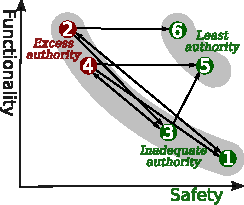
\includegraphics{seesaw-pola}}
\caption[The Evolving Authority of Active Content]{The Evolving Authority of 
Active Content. Identity-based access controls have led to thrashing between 
lost functionality and lost safety. To have both, we need to provide 
\emph{least authority}: adequate authority for desired functionality without 
excess authority which invites abube.}
  \label{fig:evo-auth}
\end{figure}

\begin{figure}[t!]
  \resizebox{\columnwidth}{!}{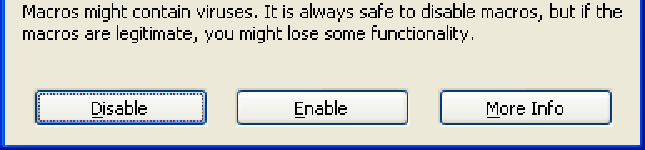
\includegraphics{dialog}}
\caption[Only Bad Choices.]{Only Bad Choices. When documents contain scripts, 
users can disable themselves from getting any work done \q{1} or enable 
scripts to destroy all their other work \q{2}.}
  \label{fig:dialog}
\end{figure}

When a document contains live interactive programs, we say it contains 
\emph{active content}. The computer industry has spent over a billion dollars 
in failed attempts to support active content. But the success of web 
apps---themselves a form of active content---demonstrates that this dream was 
worth pursuing. Unfortunately, web developers today face a maze of complex 
security mechanisms that have, so far, prevented web apps themselves from 
supporting active content. To navigate our way out of this maze, we must 
first see how we got here.

Today's desktop operating systems all use some form of identity-based access 
control~\cite{karp:abac-soa}, in which an installed application runs 
\emph{as} its user, and so is entrusted with all its user's authority. Such 
an application can provide its user all the functionality modern operating 
systems support, but at the price of being able to do anything its user may 
do. We depict this situation at~\q{2} on Figure~\ref{fig:evo-auth}. When you 
run Solitaire, it can delete all your files while playing within the rules of 
your system, without exploiting any bugs. (For the remainder of this document, 
we will ignore hazards due to implementation bugs, and explain only hazards 
due to architectural choices.)

At first, the documents handled by applications were safe passive data~\q{1}. 
Applications first supported active content by running scripts in documents 
with all of their user's authority~\qq{1}{2}. Excess authority invites abuse. 
Simply ``reading'' a malicious document would allow it to delete all your 
files. In reaction, installed office applications now encourage users to 
disable scripts (Figure~\ref{fig:dialog}) reducing content back to passive 
data~\qq{2}{1}. The failures of excess authority shown on the upper left thus 
led to the failures of inadequate authority shown on the lower right.

The web browser is itself an installed application that runs scripts in two 
contexts. Browser extensions run with all the user's authority~\q{2}. Scripts 
in web pages run sandboxed, with no authority to the user's local files. The 
browser's \emph{same origin policy}, another layer of identity-based 
control~\cite{mashupos}, provides scripts with the authority to communicate 
with their site of origin~\q{3}. Regarding both decisions, the user is 
helpless. The user has no practical way to grant a script the authority to 
edit one of the user's local files, nor can the user deny a script the 
ability to call home. So long as the user's valuable assets were local, this 
model successfully protected the user.

Web apps leverage this success. To the browser, the page on which a web app 
resides is a document, and the web app itself is simply active content within 
that document. But to the user, a web app is an application managing yet 
other documents on the user's behalf. For example, when the user interacts 
with webmail, the documents of interest are email messages. Likewise for 
groups, blogs, chat, docs and spreadsheets, wikis, and more. Let us refer to 
the documents managed by web apps as \emph{passages}, to distinguish them 
from the web pages on which they appear.

Since the user can neither grant a web app access to local files nor deny it 
the ability to call home, the only place a web app could store these passages 
is on its site of origin. The browser security model protected the user's 
local files from being harmed \emph{or used}. As users shift to using web 
apps, the assets they value come to be the passages stored at these various 
origin sites. 

To protect their user's remote passages, web apps employed yet another layer 
of identity-based controls, relying on cookies or other forms of 
authentication to identify their user. But when scripts within these passages 
ran, they would run within the web page containing the web app serving them, 
and were thereby authorized to do anything their web app could do on behalf 
of its user~\q{4}. For example, if a webmail application allowed HTML email 
messages to carry scripts, simply ``reading'' an incoming email message would 
allow it to delete your inbox. The~\qq{3}{4} transition is not a technical 
change, but a change in where the user's value resides, and thus a change in 
the user's risks. By this dynamic, failures of inadequate authority led to 
failures of excess authority.

To protect against malicious passages, some web apps do safely provide active 
content using \emph{iframes}---effectively nested web pages---at the cost of 
isolating themselves from this content~\qq{4}{3}~\cite{mashupos}. Most web 
apps \emph{sanitize} HTML content by removing all scripts, reducing content 
again to passive data~\qq{4}{1}. Existing HTML sanitizers disinfect the 
patient but leave a corpse. This recapitulates the loss of active content in 
installed office applications. Some proposals would address these next 
incremental problems by adding yet another identity-centric epicycle. Can we 
do better?

If we could start over again, we could use an authorization-centric model 
such as object-capabilities~\cite{DVH}. The object-capability alternative 
naturally supports POLA, the principle of least authority, shown in the upper 
right. An object in an object-capability language can only cause effects by 
invoking the public interfaces of objects it can reach. An invocation 
provides references to other objects as arguments, providing the invoked 
object the least authority needed to carry out these 
requests~\cite{RobustComposition}. Within these rules, active content would 
run with exactly the authority explicitly allowed by its containing document. 
Surprisingly, we can gain these benefits simply by applying a milder, 
non-lethal sanitizer.

Experience with Java~\cite{joe-e}, Scheme~\cite{rees96security}, 
OCaml~\cite{emily}, Pict~\cite{backwater}, and others demonstrates that 
existing memory safe languages often already contain an expressive 
object-capability subset. We refer to the object-capability subset of 
Javascript as \emph{Caja}. The Caja translator restricts the Javascript it 
accepts to be within this subset. This sanitized Javascript is still a 
general purpose object programming language which Javascript programmers find 
familiar, pleasant, expressive, and easy to learn and use.

Some web apps could use the Caja translator to allow active content in their 
passages~\qq{4}{5}. Other web apps could use Caja to overcome the limits of 
iframes~\qq{3}{5}. Browser extensions, which run with their user's full 
authority, could make a \emph{powerbox} available to scripts in 
pages~\cite{darpareview, stiegler:polaris, seaborn:plash, bitfrost}. A web 
app, on detecting the presence of a powerbox, could offer to edit a local 
file chosen by the user~\qq{2}{6}.

Our starting point is Javascript 1.3 as documented in the third edition of 
the EcmaScript 262 standard~\cite{ECMA-262}; hereafter \emph{ES3}. The 
remainder of this document explains the differences between Caja---the 
Javascript subset accepted by the Caja translator---and ES3. Other documents 
will explain Caja's sanitization of the remaining elements of active web 
content: HTML, CSS, and the DOM and other APIs provided by browsers to 
Javascript. We refer collectively to the subset of these accepted by the 
Caja translator as \emph{Caja web content}.


\section{Subsetting Javascript}

Caja defines a subset of Javascript both syntactically and semantically. The 
Caja translator rejects non-Caja input statically when it can. But because 
of Javascript's dynamic nature, some of Caja's restrictions cannot be 
imposed statically, so the Caja translator translates the Javascript it 
accepts into Javascript with additional runtime checks. To facilitate 
development, it is easy to write a Caja program so it can run correctly 
whether it is run as a Caja program or run directly as an untranslated 
Javascript program.

A web app (or any other Javascript-based embedding application framework) can 
be written partially in Javascript and partially in Caja. The web app loads 
the Caja runtime library, which is written in Javascript, and which is 
assumed by the Javascript output of the Caja translator. All untrusted 
scripts must be provided as Caja source code, to be verified and translated 
by the Caja translator. The translator's output is either included directly 
in the containing web page or loaded by the Caja runtime.

A loose analogy with machine and operating system architecture should help 
explain the relationships. In the analogy, the full Javascript language 
serves the role of the machine's full instruction set. Javascript's global 
scope serves the role of physical memory addresses. The I/O-capable objects 
provided to Javascript by a hosting environment, such as the DOM objects 
provided by the browser, serve the role of devices.

\begin{description}

  \item[User-mode.] By a combination of static and dynamic checks, the 
  translator allows only a safe ``user-mode'' subset of Javascript. As with 
  user-mode instructions, this subset can compute any computable function, 
  but cannot cause external effects nor sense the outside world.

  \item[Address mapping.] A package of Caja source code to be translated 
  together defines a \emph{Caja module}. All code within the same module 
  share a global scope, but distinct modules see disjoint global scopes. The 
  translator maps Caja global variable references to instead address 
  module-relative fields.

  \item[Context switching.] When Caja object A has a reference to Caja 
  object B, this should enable A to invoke B's public interface but not 
  access B's internal state. A and B should both be able to defend their 
  integrity from the other's possible misbehavior.

  \item[System calls, device drivers.] When a Caja object A invokes an 
  object B written directly in Javascript, the operations provided by B serve 
  the role of system calls. Caja protects B from A, but A is fully 
  vulnerable to B. When B is a safe wrapper around one of the host's 
  device-like objects, such as a DOM node, B also serves as a device driver.

\end{description}

A ``system call'' corresponds to a Caja object invoking a Javascript object. 
A web app that is written entirely in Javascript and provides many services 
to its Caja objects directly would be like a monolithic kernel. For 
compatibility with existing Javascript apps, we support this usage pattern 
but we don't recommend it. By analogy with kernel code at the boundary with 
untrusted code, such Javascript code needs to maintain delicate invariants 
that it is easy to get wrong.

The other extreme is analogous to a micro-kernel. The minimal necessary 
Javascript code would be the app-neutral Caja runtime itself, and a small 
app-dependent powerbox providing device drivers and initialization. All other 
services should be Caja objects to be invoked by other Caja objects. Most 
of the logic of a web app should be structured as such Caja-based services.

\subsection{Javascript specific problems}

Most of the above remarks would apply equally well were we starting from 
various other base languages. There are additional issues peculiar to 
Javascript that we must deal with. Many of these issues are also software 
engineering hazards for which Javascript programmers have developed 
defensive programming conventions. Where possible, Caja copes with these 
issues by adapting and enforcing these existing conventions.

\begin{description}

  \item[Unconstrained Properties.] Javascript objects contain 
  \emph{properties}, i.e., named fields holding references to other objects. 
  Javascript specifies that some properties are constrained to be 
  \emph{Internal}, \emph{ReadOnly}, \emph{DontEnum}, or \emph{DontDelete}. 
  Such constraints would help an object protect itself from its clients, but 
  Javascript provides no way to express these constraints in the language.
  Instead, any object defined in Javascript is freely mutated by any other
  object with access to it. 
  
  \item[Global scope.] All Javascript code executing within the same
  Javascript engine (such as a web page or iframe) implicitly share access to
  the same global scope. Therefore, in Javascript, objects cannot be isolated
  from each other.

  \item[Ambient authority.] Some base Javascript objects, such as 
  \code{Array.prototype}, are \emph{ambient}, i.e., they are implicitly 
  accessible from Caja code without any explicit grant. Put another way, 
  Caja does not give the containing Javascript app any means to deny an 
  ambient object to a Caja module. Ambient objects are thereby implicitly 
  shared by separate Caja modules loaded into the same containing app. So,
  even after the global scope problem is fixed, the mutability of these
  objects would prevent isolation.

  \item[Lack of encapsulation.] To support the ``context switching'' 
  criterion explained above, objects need to be able to encapsulate their
  private state. Javascript does provide one such mechanism: lexical variables
  captured by lexical closures. However, using this as the sole encapsulation
  mechanism for object patterns is awkward (in ways explained below).

  \item[``\code{this}'' what?] Javascript's rules for binding ``this'' depend 
  on whether a function is invoked by \emph{construction}, by \emph{method 
  call}, or by \emph{function call}. To cope with the resulting confusions, 
  Javascript programmers informally distinguish \emph{constructors}, 
  \emph{methods}, and \emph{simple functions}. Caja adapts these conventions 
  as explained below.
  
  \item[Weak static analysis.] Although Caja is less dynamic than 
  Javascript, we still assume that it is impractical to perform any 
  interesting analysis, such as type inference, both statically and safely. 
  As a result, Caja's static restrictions can only enforce simple syntactic 
  rules. Remaining restrictions must be enforced by runtime checks.
  
  \item[Fast path.] For the micro-kernel approach to be attractive, Caja's 
  extra runtime checks must not cost too much. Frequent operations, such as 
  property access using ``.'' must run close to full speed.
  
  \item[Method stealing.] In Javascript, a public method of an object can be 
  stolen by storing it as a property of a different object. The combination 
  of the ``Weak static analysis'' and ``Fast path'' criteria make it 
  impractical to prevent method stealing, so Caja must instead make stolen 
  methods useless. When a stolen method is invoked with ``this'' bound to an 
  object of the wrong type, a Caja-inserted runtime check will fail.
  
  \item[Browser compatibility.] Web content must work on widely deployed 
  browsers whether on not these browsers strictly conform to the relevant 
  standards. At the time of this writing, the plausible baseline platform is 
  the intersection of ES3, Firefox 1.5, Internet Explorer 6, Opera 8.5, 
  Safari 3, and their successors. Fortunately, these browsers do conform 
  quite closely to ES3. Later versions of Caja may specify larger subsets of 
  EC3.
  
  \item[Silent errors.] In Javascript, various operations, such as setting a 
  ReadOnly property, fail silently rather than throwing an error. Program 
  logic then proceeds along normal control flow paths premised on the 
  assumption that these operations succeeded, leading to inconsistency. To 
  program defensively in the face of this hazard, every assignment would be 
  followed by a ``did it really happen?'' test. This would render programs 
  unreadable and unmaintainable. Where practical, Caja deviates from 
  standard Javascript by throwing errors rather than failing silently. Caja 
  is therefore only a subset of Javascript in a limited sense: While a Caja 
  program proceeds on non-exceptional control flow paths, it executes within 
  Javascript's semantics.
  
\end{description}

This last point about ``Silent errors'' is another reason to avoid the 
monolithic kernel approach. Web apps in untranslated Javascript are 
vulnerable to any malicious active content that finds a way to provoke a 
silent error and exploit the resulting inconsistency.

\subsection{Definitions}

To explain the restrictions Caja imposes on Javascript, we need some
definitions. 

\begin{description}

  \item[JSON Container.] An object whose prototype's ``\code{constructor}'' 
  property is \code{Array} or \code{Object}, i.e., under normal conditions, 
  an object inheriting directly from \code{Array.prototype} or 
  \code{Object.prototype}.

  \item[Constructed object.] Any object that's not a JSON container, which 
  must therefore have been constructed by calling ``\code{new}'' on a 
  consructor other than \code{Array} or \code{Object}. 

  \item[Simple functions.] A function whose body does not mention 
  ``\code{this}'' is a \emph{simple function}. A simple function can be 
  either named or anonymous. By convention, a simple function's name should 
  begin with a lower case letter, but this is not enforced. A simple function 
  can be invoked by \emph{as a function} (\code{foo(a\ldots)}), \emph{as a 
  method} (\code{foo.id(a\ldots)}), or \emph{as a constructor} (\code{new 
  Foo(a\ldots)}).
    
  \item[Constructors.] A named function whose body mentions ``\code{this}'' 
  is a \emph{constructor}. By convention, a constructor's name should begin 
  with an upper case letter, but this is not enforced. A constructor can only 
  be invoked by construction, i.e., by a call using the ``\code{new}'' 
  keyword.
    
  \item[Methods.] An anonymous function whose body mentions ``\code{this}'' 
  is a \emph{method}. A method definition may only appear in prototype 
  property initializations. By convention, the property name associated with 
  a method should begin with a lower case letter, but this is not enforced. A 
  method may only be called by a method call binding ``\code{this}'' to an 
  already-constructed object of the expected type. (See ``Method stealing" 
  above.)

\end{description}

The purpose of most of Caja's restrictions is to enable a reference to a 
constructed object to serve as a capability.

\subsection{Static restrictions}

Any source code statically accepted by the Caja translator is \emph{verified 
Caja program text}. The presence of the following syntactic elements causes 
an alleged Caja program text to instead be statically rejected.

\begin{description}

    \item[Stable language.] Virtually any input which should be statically 
    rejected by ES3 is forbidden, even if it would be allowed by a target 
    browser or later Javascript specifications. This includes any use of 
    keywords reserved in ES3. But we reserve the right to include 
    \emph{de-facto extensions} to ES3 as explained below.
    
    \item[De-facto extensions.] As we identify widely supported extensions of 
    ES3 that we can accept as input, but still translate to conforming 
    EcmaScript on output, we may add these to Caja. For example, we are 
    currently considering allowing backslash as a line continuation 
    character, since this is allowed by virtually all Javascript 
    implementations and can be trivially translated to correct ES3.

    \item[Without ``\code{with}''.] The ``\code{with}'' keyword is forbidden. 
    Because of the scope confusion it causes, ``\code{with}'' is a widely 
    hated and avoided feature that would be a lot of trouble to support 
    safely.

    \item[Beware unicode.] Non-Latin-1 characters are forbidden for now in 
    source text outside of string literals. Some of these create parsing 
    problems on some widely deployed Javascript platforms. Prohibiting these 
    protects against some char-encoding attacks. We expect to relax this 
    restriction once we know how to do so safely.

    \item[Internal properties.] An identifier ending in a single underscore 
    may be used only to name Internal properties. It may appear only after a 
    ``\code{this.}''.

    \item[Forbidden names.] An identifier ending with a double underscore is 
    forbidden, either as a variable name or a property name. We reserve the 
    triple underscore for use by the Caja translator output and the Caja 
    runtime code. Firefox reserves use of the double underscore for itself.
    
    \item[RegExpr syntax.] In Javascript implementations, the pattern syntax 
    is often optimized into a static object with mutable state, violating 
    isolation. Caja translates the \code{/pattern/} syntax to \code{new 
    RegExp("pattern")}.
        
\end{description}

\begin{figure}
\begin{alltt}
function F(a\ldots)\{\ldots\}
F.prototype.mname = /*method or function*/;
F.prototype.mname = /*expr with no F*/;
\ldots
F.sname = /*function or expr with no F*/;
\ldots
/*Generate \_\_\_.freeze(F.prototype); here*/
/*Generate \_\_\_.freeze(F); here*/
/*first use of F*/
\end{alltt}

\caption[Initializing the Default Prototype]{Initializing the Default
Prototype. The normal syntactic pattern for expressing class-like code is
accepted, so long as all behavior definition happens before the first use of
F. The \emph{mnames} would typically be method names. The \emph{snames} name
static members, to be accessed off the constructor.}
\label{fig:use-proto}
\end{figure}


\begin{figure}
\begin{alltt}
// Shorthand using:
// caja.def(F,Sup,opt_members,opt_statics);

function F(a\ldots)\{
  F.Super.call(this,b\ldots); //optional
  \ldots
\}
caja.def(F, G,\ \{
  mname: /*method, function, or expr*/),
  \ldots
\},\ \{
  sname: /*function or expr*/),
  \ldots
\});
/*first use of F*/
\end{alltt}

\caption[Shorthand.]{Shorthand. As a convenience, the translator recognizes 
this pattern as still defining \emph{F} rather than using it. \code{caja.def}
initializes \code{F.Super = G}, sets up the normal inheritance relationship
between F and G, and freezes F.prototype and F.}
\label{fig:shorthand}
\end{figure}


\begin{figure}
\begin{alltt}
function Point(x, y)\ \{
  this.x\_ = x;
  this.y\_ = y;
\};
Point.prototype.toString = function()\ \{ 
  return "<" + this.x\_ + "," + 
               this.y\_ + ">"; 
\};
Point.prototype.getX = function()\ \{ 
  return this.x\_; 
\};
Point.prototype.getY = function()\ \{ 
  return this.y\_; 
\};
Point.prototype.add = function(other)\ \{
  return new Point(
    this.x\_ + other.getX(),
    this.y\_ + other.getY());
\};

var pt = new Point(3, 5);
\end{alltt}
\caption[Generic Point Example.]{Generic Point Example.}
\label{fig:generic-point}
\end{figure}


\begin{figure}
\begin{alltt}
function Point(x, y)\ \{
  this.x\_ = x;
  this.y\_ = y;
\};
Caja.def(Point, Object,\ \{
  toString: function()\ \{ 
    return "<" + this.x\_ + "," + 
                 this.y\_ + ">"; 
  \},
  getX: function()\ \{ return this.x\_; \},
  getY: function()\ \{ return this.y\_; \},
  add: function(other)\ \{
    return new Point(
      this.x\_ + other.getX(),
      this.y\_ + other.getY());
  \}
\});

var pt = new Point(3, 5);
\end{alltt}
\caption[Brief Point Example.]{Brief Point Example.}
\label{fig:brief-point}
\end{figure}

Although constructors are normally frozen and the ``\code{prototype}'' 
property of functions is generally not settable, we allow at least the 
patterns shown in Figures~\ref{fig:use-proto} and~\ref{fig:shorthand} for 
declaring a constructor, initializing it, and initializing its prototype. 
Figures~\ref{fig:generic-point} and~\ref{fig:brief-point} show a familiar 
example expressed in these patterns.

The first argument to ``\code{Caja.def}'' may be the prototype only of a 
fresh definition of F. None of these initialization may make any other use of 
F or F.prototype. All initialization of F and its prototype will therefore 
precede any use of F. This means, in effect, that the assignments above can 
be considered declarative initializations rather than mutations. The mention 
of ``\code{Point}'' within the ``\code{add}'' method is not considered a 
too-early usage of ``\code{Point}'' since it occurs only within a method body 
that cannot be executed too early.

Claim: \emph{No Caja program can cause an observable mutation of an object
Caja considers frozen.}


\subsection{Outer scope restrictions}

In Javascript, all code loaded into the same Javascript execution environment 
shares a common mutable global scope. To avoid confusion, we refer to the 
corresponding concept in Caja as the \emph{outer scope}. The Caja outer scope
 comes in two layers:

Caja's \emph{shared outer scope} contains the subset of the standard ES3 
global scope that we deem to be safe. This includes all the objects and 
properties defined by that standard, with the following caveats. Unless 
stated otherwise, all the objects in this outer scope are transitively 
immutable, so that they provide no ambient authority to objects defined 
within this scope. The shared outer scope itself is frozen.

Each instantiation of a Caja module is a separate plugin. Each plugin 
executes with a new \emph{per-plugin outer scope} which is mutable and 
inherits from Caja's shared outer scope. Therefore, all objects within the 
same plugin can implicitly communicate and interfere with each other. 
However, \emph{claim: two separate plugins, even if they instantiate the same 
module, are isolated from each other.}

\begin{description}

    \item[eval] The Caja global scope has no ``\code{eval}'' function. 
    Instead, the ``\code{Caja.eval}'' method will evaluate Caja source code 
    with an explicitly provided set of variable bindings to serve as its 
    initial global scope, as explained below.
    
    \item[Function] The Javascript \code{Function} constructor is absent from 
    the default Caja outer scope, and must not be available in Caja. 

    Unfortunately, \code{Function} is unsafe even when invoked as a normal 
    function, and we're currently hoping to stop protecting normal function 
    calls with a runtime check. \emph{Claim: Even without the runtime check 
    on normal function calls, the rest of the restrictions in this document 
    together make \code{Function} uncreachable from Caja programs.}
    
    \item[function.constructor] The Javascript \code{constructor} property of 
    functions is absent from Caja.

    \item[new Date()] In Javascript, ``\code{new Date()}''  gives ambient 
    access to the current date and time, in violation of object-capability 
    rules as well as dependency injection discipline. \code{Date} is 
    therefore a member of the global scope which is not actually immutable. 
    Further, this ambient access to the current time provides a timing 
    channel, further impeding any attempts to stem the leakage of bits over 
    covert channels. Nevertheless, despite these concerns, because it 
    provides only a read-only channel for sensing the world, Caja provides 
    the Javascript \code{Date} constructor to Caja programs.

    \item[Math.random()] The Javascript \code{Math.random} method is not even 
    read-only. The ES3 standard places no obligations regarding quality of the
    randomness produced. In particular, an implementation could conform to ES3
    and still leak to a given caller of \code{Math.random()} the ability to
    infer how many previous times it had been called. Nevertheless, Caja
    provides the Javascript \code{Math.random} method to Caja programs. We
    recommend that Javascript platform providers provide good enough
    randomness that this method doesn't serve as an information channel
    between otherwise-isolated plugins.
    
\end{description}

\subsection{Dynamic restrictions}

TODO To be written

\section{The Caja Library}

TODO To be written

\section{Examples}

TODO To be written

\section{The Caja translator}

TODO To be written

\section{Conclusions}

TODO To be written

\section{Acknowledgements}

We thank 
Dirk Balfanz,
Doug Crockford.

\appendix

\section{Tables}

\begin{table*}
\begin{tabular}{ll}
  Caja expression    & translates to ES3 code equivalent to\\ 
  \hline
  \code{with}        & /*rejected*/ \\
  \hline
  \code{this.id\_\_} & /*rejected in all positions*/ \\
  \code{foo.id\_}    & /*rejected in all positions*/ \\      
  \code{local\_\_}   & /*rejected in all positions*/ \\        
  \code{glob\_}      & /*rejected in all positions*/ \\        
  \hline
  \code{this.id\_}   & /*unaltered*/ \\
  \code{this.id}
    & \code{this.id\_canRead\_\_\_ ?\ this.id :\ \_\_\_.readProp(this,"id")}\\
  \code{foo.id}
    & \code{foo.id\_canRead\_\_\_ ?\ foo.id :\ \_\_\_.readPub(foo,"id")} \\
  \code{this[bar]}   & \code{\_\_\_.readProp(this,bar)} \\
  \code{foo[bar]}    & \code{\_\_\_.readPub(foo,bar)}  \\
  \code{glob}        & \code{\_\_\_OUTERS\_\_\_.glob} \\
  \hline
  \code{bar in this}           
    & \code{(bar in this) \&\& \_\_\_.canReadProp(this,bar)} \\
  \code{bar in foo}            
    & \code{(bar in foo) \&\& \_\_\_.canReadPub(foo,bar)} \\
  \code{for (key in this)\ \{\ldots\}} 
    &\code{for (key in this)\ \{if (canEnumProp(this,key))\ \{\ldots\}\}}\\
  \code{for (key in foo)\ \{\ldots\}}  
    & \code{for (key in foo)\ \{if (canEnumPub(foo,key))\ \{\ldots\}\}} \\
  \hline
  \code{this.id = baz}    
    & \code{this.id\_canSet\_\_\_ ?\ (this.id = baz) :\
\_\_\_.setProp(this,"id",baz)} \\
  \code{foo.id = baz}     
    & \code{foo.id\_canSet\_\_\_ ?\ (foo.id = baz) :\
\_\_\_.setPub(foo,"id",baz)} \\
  \code{this[bar] = baz}  & \code{\_\_\_.setProp(this,bar,baz)} \\
  \code{foo[bar] = baz}   & \code{\_\_\_.setPub(foo,bar,baz)} \\
  \code{glob = baz}       & \code{\_\_\_OUTERS\_\_\_.glob = baz} \\
  \code{var glob = baz}   & \code{\_\_\_OUTERS\_\_\_.glob = baz} \\
  \code{var glob}         & \code{\_\_\_OUTERS\_\_\_.glob = undefined} \\
  \hline               
  \code{delete this.id}   & \code{\_\_\_.deleteProp(this,"id")} \\
  \code{delete foo.id}    & \code{\_\_\_.deletePub(foo,"id")} \\
  \code{delete this[bar]} & \code{\_\_\_.deleteProp(this,bar)} \\
  \code{delete foo[bar]}  & \code{\_\_\_.deletePub(foo,bar)} \\
  \code{delete glob}      
         & \code{\_\_\_.require(delete \_\_\_OUTERS\_\_\_.glob,\ldots)} \\
\end{tabular}

\caption[Translating Property Access]{Translating Property Access. Under the 
assumption that the Caja runtime environment is as specified, the Caja 
translator generates translations equivalent to those specified above, but 
inlined and optimized where possible. The meaning of translating is thereby 
determined by the specification of these entry points into the Caja runtime 
library. Where we show a translation apparently duplicating an expression,
the translator instead introduces temporary variables as needed so that
each expression evaluates exactly as many times and in the same order as in
the original.}
\label{tab:prop-xlate}
\end{table*}


\begin{table*}
\begin{tabular}{ll}
  Caja expression   & translates to ES3 code equivalent to\\ 
  \hline
                 & \code{\_\_\_.module(function(\_\_\_OUTERS\_\_\_)\ \{} \\
  /*caja module body*/      
                 & \code{\ \ } /*translated module body*/ \\
                 & \code{\});} \\
  \hline
  \code{new F(a\ldots)}     & \code{\_\_\_.callNew(F,[a\ldots])} \\
  \code{this.id\_(a\ldots)} & /*unaltered*/ \\
  \code{this.id(a\ldots)} 
                 & \code{\_\_\_.readProp(this,"id").call(this,a\ldots)} \\
  \code{foo.id(a\ldots)}  
                 & \code{\_\_\_.readPub(foo,"id").call(foo,a\ldots)} \\
  \code{foo(a\ldots)}       & \code{foo.call(\_\_\_.USELESS,a\ldots)} \\
  \hline
  \code{function F(a\ldots)\ \{}  
                 & \code{var F = \_\_\_.ctor(function(a\ldots)\ \{} \\
                 & \code{\ \ \_\_\_.enterDerived(F,this);} \\
  \code{\ \ F.Super.call(this,b\ldots);}
                 & \code{\ \ F.Super.call(this,b\ldots);} \\
  \code{\ \ \ldots this\ldots\}}
                 & \code{\ \ \ldots this\ldots\})} \\
  \hline
  \code{function F(a\ldots)\ \{}  
                 & \code{var F = \_\_\_.ctor(function(a\ldots)\ \{} \\
                 & \code{\ \ \_\_\_.enterBase(F,this);}\\
  \code{\ \ \ldots this\ldots\}}
                 & \code{\ \ \ldots this\ldots\})}\\
  \hline
  \code{function(a\ldots)\ \{}    
                 & \code{\_\_\_.method(F,function(a\ldots)\ \{} \\
                 & \code{\ \ \_\_\_.enterMethod(arguments.callee,this);}\\
  \code{\ \ \ldots this\ldots\}}
                 & \code{\ \ \ldots this\ldots\})}\\
  
  \hline
  \code{function foo(a\ldots)\ \{}   
                 & \code{var foo = \_\_\_.freeze(function(a\ldots)\ \{} \\
  \code{\ \ \ldots\}}          
                 & \code{\ \ \ldots; return undefined;\})} \\
  
  \code{function(a\ldots)\ \{}
                 & \code{\_\_\_.freeze(function(a\ldots)\ \{} \\
  \code{\ \ \ldots\}}          
                 & \code{\ \ \ldots; return undefined;\})} \\
  \hline
  \code{arguments.callee}   & /*unaltered, to allow anonymous recursion*/ \\
  \code{\ldots arguments\ldots} 
     &\code{var \_\_\_args\_\_\_ = \_\_\_.args(arguments);}\\
                 & \code{\ldots \_\_\_args\_\_\_\ldots} \\
  \hline
  \code{/pattern/} & \code{new RegExp("pattern")}
\end{tabular}

\caption[Translating Callers and Callees]{Translating Callers and Callees.
A translated Caja module can be loaded/evaled once, creating an anonymous
plugin-maker function. Each time the plugin-maker representing a module is
called, it makes a new plugin. Unless their creator puts them in contact, even
plugins made by the same plugin-maker are isolated from each other. A function
that falls off the end is rewritten to return \code{undefined} explicitly, in
case it is called as a constructor.}
\label{tab:call-xlate}
\end{table*}


\begin{table*}
\begin{tabular}{ll}
  Methods of \code{\_\_\_}  & method body \\ 
  \hline 
  \code{require(test,complaint)}
       & \code{if (test)\ \{ return true; \}} \\
       & \code{throw new CajaRuntimeError(complaint);} \\
  \hline 
  \code{hasOwnProp(obj,name)} 
       & \code{return Object.prototype.hasOwnProperty.call(obj,name);} \\
  \code{isJSONContainer(obj)} 
       & \code{var Constr = directConstructor(obj);} \\
       & \code{return Constr === Object || Constr === Array;} \\ 
  \code{isFrozen(obj)} 
       & \code{return hasOwnProp(obj,"\_\_\_FROZEN\_\_\_");} \\
  \code{freeze(obj)}*
       & \code{for (k in obj)\ \{} \\
       & \code{\ \ if (endsWith(k,"\_canSet\_\_\_"))\ \{ obj[k] = false; \}} \\
       & \code{\}} \\
       & \code{obj.\_\_\_FROZEN\_\_\_ = true;} \\
       & \code{return obj;} \\
  \hline
  \code{canRead(obj,name)}  & \code{return !!obj[name+"\_canRead\_\_\_"];} \\
  \code{canEnum(obj,name)}  & \code{return !!obj[name+"\_canEnum\_\_\_"];} \\
  \code{canSet(obj,name)}   & \code{return !!obj[name+"\_canSet\_\_\_"];} \\
  \hline
  \code{allowRead(obj,name)}* 
       & \code{return obj[name+"\_canRead\_\_\_"] = true;} \\
  \code{allowEnum(obj,name)}* 
       & \code{return obj[name+"\_canEnum\_\_\_"] = allowRead(obj,name);} \\
  \code{allowSet(obj,name)}* & \code{require(!isFrozen(obj),\ldots);} \\
       & \code{return obj[name+"\_canSet\_\_\_"] = allowEnum(obj,name);} \\
  \hline
  \code{isCtor(Constr)}
       & \code{return !!Constr.\_\_\_CONSTRUCTOR\_\_\_;} \\
  \code{isMethod(meth)}
       & \code{return !!meth.\_\_\_METHOD\_OF\_\_\_;} \\
  \code{isMethodOf(meth,receiver)}
       & \code{if (isMethod(meth))\ \{} \\
       & \code{\ \ return receiver instanceof meth.\_\_\_METHOD\_OF\_\_\_;} \\
       & \code{\} else\ \{ return !isCtor(meth); \}} \\
  \hline
  \code{ctor(Constr)}*
       & \code{require(typeof Constr === "function",\ldots);} \\
       & \code{Constr.\_\_\_CONSTRUCTOR\_\_\_ = true;} \\
       & \code{return Constr;} /*translator freezes Constr later*/ \\
  \code{method(Constr,meth)}*
       & \code{require(typeof meth === "function",\ldots);} \\
       & \code{require(isCtor(Constr),\ldots);} \\
       & \code{meth.\_\_\_METHOD\_OF\_\_\_ = Constr;} \\
       & \code{return freeze(meth);} \\
  \code{wrapMethod(Constr,name,meth)}*
       & \code{require(name in Constr.prototype,\ldots);}\\
       & \code{meth.\_\_\_ORIGINAL\_\_\_ = Constr.prototype[name];}\\
       & \code{Constr.prototype[name] = meth;}\\
       & \code{return method(Constr,meth);}\\
  \hline
  \code{makeRaw(Constr)}
       & \code{function F()\ \{ this.\_\_\_RAW\_\_\_ = true; \}} \\
       & \code{F.prototype = Constr.prototype;} \\
       & \code{return new F();} \\
  \code{cookIfRaw(obj)}
       & \code{return delete obj.\_\_\_RAW\_\_\_;} \\
\end{tabular}

\caption[Hidden Attributes.]{Hidden Attributes. These methods handle the 
concrete representations of object and property attributes. Only the methods 
marked with a * should called by Javascript code during initialization of the 
embedding app, in order to express taming decisions. All objects that are 
reachable from the ES3 shared scope should be frozen, so that this shared 
scope becomes transitively read-only to all Caja code.}
\label{tab:hide-attr}
\end{table*}


\begin{table*}
\begin{tabular}{ll}
  Methods of \code{\_\_\_}  & method body \\ 
  \hline 
  \code{canReadProp(self,name)}
       & \code{if (endWith(name,"\_\_"))\ \{ return false; \}} \\
       & \code{return canRead(self,name);} \\
  \code{readProp(self,name)}
       & \code{return canReadProp(self,name) ?\ self[name] :\ undefined;} \\
  \code{canReadPub(obj,name)}
       & \code{if (endWith(name,"\_"))\ \{ return false; \}} \\
       & \code{if (canRead(obj,name))\ \{ return true; \}} \\
       & \code{if (!isJSONContainer(obj))\ \{ return false; \}} \\
       & \code{if (!hasOwnProp(obj,name))\ \{ return false; \}} \\
       & \code{return allowRead(obj,name);} /*memoize*/ \\
  \code{readPub(obj,name)}
       & \code{return canReadPub(obj,name) ?\ obj[name] :\ undefined;} \\
  \hline
  \code{canEnumProp(self,name)} 
       & \code{if (endWith(name,"\_\_"))\ \{ return false; \}} \\
       & \code{return canEnum(self,name);} \\
  \code{canEnumPub(obj,name)}
       & \code{if (endWith(name,"\_\_"))\ \{ return false; \}} \\
       & \code{if (canEnum(obj,name))\ \{ return true; \}} \\
       & \code{if (!isJSONContainer(obj))\ \{ return false; \}} \\
       & \code{if (!hasOwnProp(obj,name))\ \{ return false; \}} \\
       & \code{return allowEnum(obj,name);} /*memoize*/ \\
  \hline
  \code{canSetProp(self,name)}
       & \code{if (endWith(name,"\_\_"))\ \{ return false; \}} \\
       & \code{if (canSet(self,name))\ \{ return true; \}} \\
       & \code{return !isFrozen(self);} \\
  \code{setProp(self,name,val)}
       & \code{require(canSetProp(self,name),\ldots);} \\
       & \code{allowSet(self,name);} /*grant*/ \\
       & \code{return self[name] = val;} \\
  \code{canSetPub(obj,name)}
       & \code{if (endWith(name,"\_"))\ \{ return false; \}} \\
       & \code{if (canSet(obj,name))\ \{ return true; \}} \\
       & \code{return !isFrozen(obj) \&\& isJSONContainer(obj);} \\
  \code{setPub(obj,name,val)}
       & \code{require(canSetPub(obj,name),\ldots);} \\
       & \code{allowSet(obj,name);} /*grant*/ \\
       & \code{return obj[name] = val;} \\
  \hline               
  \code{deleteProp(self,name)} 
       & \code{require(canSetProp(self,name),\ldots);} \\
       & /*XXX Bookkeeping yet to be determined*/ \\
       & \code{return require(delete self[name],\ldots);} \\
  \code{deletePub(obj,name)} 
       & \code{require(canSetPub(obj,name),\ldots);} \\
       & \code{require(isJSONContainer(obj),\ldots);} \\
       & /*XXX Bookkeeping yet to be determined*/ \\
       & \code{return require(delete obj[name],\ldots);}
\end{tabular}

\caption[Property Access.]{Property Access. The calls to \code{allowRead} and
\code{allowEnum} merely memoize a query result. The calls to \code{allowSet}
track the implications of side effects.}
\label{tab:prop-access}
\end{table*}


\begin{table*}
\begin{tabular}{ll}
  Methods of \code{\_\_\_}  & method body \\ 
  \hline 
  \code{callNew(Constr,args)} 
       & \code{require(!isMethod(Constr),\ldots);} \\
       & \code{var result = Constr.apply(makeRaw(Constr), args);} \\
       & \code{cookIfRaw(result);} /*remove RAW flag as soon as possible*/ \\
       & \code{return result;} \\
  \hline
  \code{enterBase(Constr,self)}
       & \code{require(self instanceof Constr),\ldots);} \\
       & \code{require(cookIfRaw(self),\ldots);} \\
  \code{enterDerived(Constr,self)}
       & \code{require(self instanceof Constr),\ldots);} \\
       & \code{require(isRaw(self),\ldots);} \\
  \code{enterMethod(meth,self)}
       & \code{require(isMethodOf(meth,self),\ldots);} \\
       & \code{require(!cookIfRaw(self),\ldots);} \\
  \hline
  \code{args(original)}
       & \code{return freeze(Array.prototype.slice.call(original,0));}
\end{tabular}

\caption[Context Switching.]{Context Switching. Javascript code must not use 
Javascript's \code{new} on Caja code. Beyond this, no matter whether caller 
or callee is in Javascript or Caja, a constructor can be called as 
a constructor using \code{new}, a method can be called as a method, and 
a function can be called as a function, method, or constructor.}
\label{tab:context-switching}
\end{table*}


\begin{table*}
\begin{tabular}{lll}
  Global ES3 non-constructor & Property                   & Taming \\
  \hline
  \code{NaN}                &                             & ok \\
  \code{Infinity}           &                             & ok \\
  \code{undefined}          &                             & ok \\
  \code{eval}               &                             & hidden \\
  \code{parseInt}           &                             & ok \\
  \code{parseFloat}         &                             & ok \\
  \code{isNaN}              &                             & ok \\
  \code{isFinite}           &                             & ok \\
  \hline
  \code{decodeURI}          &                             & ok \\
  \code{decodeURIComponent} &                             & ok \\
  \code{encodeURI}          &                             & ok \\
  \code{encodeURIComponent} &                             & ok \\
  \hline
  \code{Math}               &                             & ok \\  
                            & \code{random}               & ok* \\
                            &           all others in ES3 & ok \\
\end{tabular}

\caption[Taming ES3 Global Non-Constructors.]{Taming ES3 Global 
Non-Constructors. Except for \code{eval}, all non-constructors specified by 
ES3 are visible in Caja's outer scope as immutable objects. Note that 
\code{Math.random} is not actually immutable, and therefore neither is 
\code{Math} nor Caja's outer scope itself. We allow it anyway for reasons
explained in the text.}
\label{tab:taming-es3}
\end{table*}
  
\begin{table*}
\begin{tabular}{lll}
  Global ES3 constructor         & Property                    & Taming \\
  \hline 
  constructor                    &                             & default ok \\
  constructor\code{.prototype}   &                             & default ok \\
                                 & \code{constructor}          & hidden \\
                                 & \code{toString}             & default ok \\
                                 & \code{toLocaleString}       & default ok \\
                                 & \code{valueOf}              & default ok \\
  instances                      & \code{length}               & default ok \\
  \hline
  \code{Object.prototype}        & \code{hasOwnProperty}       & wrapped \\
                                 & \code{isPrototypeOf}        & ok \\
                                 & \code{propertyIsEnumerable} & wrapped \\
  \hline
  \code{Function}                &                             & hidden \\
  \code{Function.prototype}      &                             & ok? \\
                                 & \code{apply}                & wrapped \\
                                 & \code{call}                 & wrapped \\
  instances                      & \code{prototype}            & ok \\
                                 & \code{length}               & ok \\
  \hline
  \code{Array.prototype}         & \code{concat}               & ok \\
                                 & \code{join}                 & ok \\
                                 & \code{pop}                  & wrapped \\
                                 & \code{push}                 & wrapped \\
                                 & \code{reverse}              & wrapped \\
                                 & \code{shift}                & wrapped \\
                                 & \code{slice}                & ok \\
                                 & \code{sort}                 & wrapped \\
                                 & \code{splice}               & wrapped \\
                                 & \code{unshift}              & wrapped \\
                                 & \code{indexOf}              & added \\
                                 & \code{lastIndexOf}          & added \\
  \hline
  \code{String}                  & \code{fromCharCode}         & ok \\
  \code{String.prototype}        & \code{match}                & wrapped \\
                                 & \code{replace}              & wrapped \\
                                 & \code{search}               & wrapped \\
                                 & \code{split}                & wrapped \\
                                 &           all others in ES3 & ok \\
\end{tabular}

\caption[Taming ES3 Global Constructors, Part 1.]{Taming ES3 Global
Constructors, Part 1. The first section above shows the taming
decisions that apply by default to global ES3 constructors, their prototypes,
and their instances, unless stated otherwise in a specific table entry. The
\code{Array} methods are wrapped to ensure they don't violate Caja's
mutability constraints.}
\label{tab:taming-es3-1}
\end{table*}



\begin{table*}
\begin{tabular}{lll}
  Global ES3 constructor         & Property                    & Taming \\
  \hline 
  \code{Boolean}                 &                             & ok \\
  \hline
  \code{Number}                  & \code{MAX\_VALUE}           & ok \\
                                 & \code{MIN\_VALUE}           & ok \\
                                 & \code{NaN}                  & ok \\
                                 & \code{NEGATIVE\_INFINITY}   & ok \\
                                 & \code{POSITIVE\_INFINITY}   & ok \\
  \code{Number.prototype}        & \code{toFixed}              & ok \\
                                 & \code{toExponential}        & ok \\
                                 & \code{toPrecision}          & ok \\
  \hline
  \code{Date}                    &                             & ok* \\
                                 & \code{parse}                & ok \\
                                 & \code{UTC}                  & ok \\
  \code{Date.prototype}          & \code{to*String} all in ES3 & ok \\
                                 & \code{toISOString}          & added \\
                                 & \code{get*}      all in ES3 & ok \\
                                 & \code{set*}      all in ES3 & wrapped \\
  \hline
  \code{RegExp.prototype}        & \code{exec}                 & wrapped \\
                                 & \code{test}                 & wrapped \\
  instances                      & \code{source}               & ok \\
                                 & \code{global}               & ok \\
                                 & \code{ignoreCase}           & ok \\
                                 & \code{multiline}            & ok \\
                                 & \code{lastIndex}            & ok \\
  \hline 
  \code{Error.prototype}         & \code{name}                 & ok \\
                                 & \code{message}              & ok \\
  \code{*Error}                  &                  all in ES3 & ok \\
  \code{*Error.prototype}        &                  all in ES3 & ok \\
  
\end{tabular}

\caption[Taming ES3 Global Constructors, Part 2.]{Taming ES3 Global
Constructors, Part 2. The \code{Date} constructor itself gives ambient
read-only access to the current time, and is therefore not immutable.
We allow it anyway for reasons explained in the text.} 

\label{tab:taming-es3-1}
\end{table*}





\bibliographystyle{abbrv}
\bibliography{common}

\end{document}
